\section{Improving the SCD network with the DDS}
\label{sec:ddstcv}
The strict real-time requirements of a sophisticated control system such as the SCD, described in \Cref{sec:scd}, ask for an implementation that is designed and configured for the task at hand in any of its parts. Operating system kernels are compiled with patches that enable fine-grained real-time task scheduling policies. The software is written with frameworks that guarantee real-time execution, such as MARTe2. The hardware is powerful enough to handle the computational load of the control algorithms, reserving to them all the system resources they require (\emph{e.g.}, CPU, RAM, PCI bandwidth) in a deterministic fashion, cutting out every other task including system ones. When sampling times get to the microsecond precision declared in \Cref{sec:scd}, every component of the system has to be carefully considered.

In this scenario, things are a bit complicated by the fact that SCD is \emph{distributed} in the sense that has been described in \Cref{ch:intro}. It is not a single system but an interconnection of multiple computational nodes each executing a predefined set of tasks encoded in specific software subsystem, also interfacing with dedicated hardware components when necessary. Each node cannot perform its tasks alone: for example, control nodes 02 and 03 cannot actuate the coil power supplies properly without the real-time data provided by the plasma equilibrium reconstruction, which runs on nodes 05 and 06, which in turn need the data from the plasma diagnostics running on other nodes. By this description, it is clear how the communication infrastructure among the nodes has to be carefully designed and implemented to guarantee the real-time performance of the whole system. It requires a technology that makes it fast, deterministic, and reliable.

Currently (see \cite{galperti_overview_2024}), the SCD nodes are interconnected by a real-time fiber optic network that implements a \emph{reflective memory} (RFM). In essence, reflective memories are shared memory systems that allow multiple machines to share a data area. The implementation of the RFM usually consists of a high-speed connection medium, in this case an optic fiber connection, and dedicated network cards to install on the machines forming the network. These cards contain the actual data area and their device drivers map that area within the main memory of the host machine. The RFM implementation is such that each local copy of the shared data area is kept coherent with the others, so that every write operation is propagated to all the other copies. The timings that these operations might take can be very tight but, most importantly, they are deterministic. This makes the RFM a suitable technology for this kind of application scenario.

The RFM technology has been commercially available since the 1980s and SCD adopts Abaco Systems network cards \cite{abaco_systems_pcie-5565rc_nodate}. As stated in \Cref{sec:scd}, these cards and their fiber optic interconnection allow SCD to maintain sub-microsecond latencies when transferring data among the nodes with a throughput up to \SI{170}{\mega\byte/\second}. This implementation has allowed SCD to perform well in the last decade but it is now showing some concerning issues, especially in terms of scalability and maintainability. First, as stated in \cite{abaco_systems_pcie-5565rc_nodate}, the Abaco cards are reaching their End Of Life (EOL) status with a limited production phase started in 2022. This, together with their high price (around 8.000€/card), is creating procurement concerns at SPC for such a critical component of the SCD. Secondly, the throughput of the RFM network is not enough to handle the increasing amount of data that the SCD nodes have to exchange. New diagnostics are being evaluated and added each year, with some of them capable of generating considerable amounts of data, such as the MANTIS camera system on Node 10. The problem becomes clear when one notes that the data area is shared among \emph{all} the nodes, so they have to use that space to exchange data coming from every device and subsystem all at the same time. Despite some access policies that have been implemented to deal with this without increasing latencies (see, again, \cite{galperti_overview_2024}), a saturation point has been reached and new diagnostics such as bolometry cannot currently be used in real-time control because their data cannot be shared among the nodes.

To enable further upgrades to the SCD increasing TCV's experimental capabilities, as well as to avoid ending up relying on an EOL component, a replacement solution for the RFM network has become necessary. Various criteria have been applied to its selection, including the cost-effectiveness of relying again on dedicated hardware components when common network hardware such as Ethernet has evolved so much in the meantime, guaranteeing bandwidths that were simply unthinkable at the time in which the reflective memory was invented. Ideally, a properly configured, reserved Ethernet network is enough if it is driven by a software protocol that is able to guarantee the same determinism and low latencies of the RFM. The Data Distribution Service, introduced in \Cref{sec:dds}, is a candidate technology that can provide these features and has been selected as a replacement for the RFM network in the SCD.

This section describes the design of a software component for the SCD architecture that integrates the DDS middleware for communication purposes. Then, it presents some results of its application on SCD nodes, showing promising performance that motivated the decision to proceed with the integration of the DDS in the SCD. These results prove how the distributed technologies that constitute the base of the DUA framework presented in \Cref{ch:dua} can be applied successfully even to a different context such as the control system of a tokamak device.

\subsection{Design of the DDSDataSource for the MARTe2 framework}
\label{sec:ddsdatasource}
As every hardware component of the SCD architecture, the reflective memory is integrated with it by the means that the MARTe2 framework provides. Recalling the overview of MARTe2 given in \Cref{sec:related_work_marte2}, the software components dedicated to the integration of specific hardware are called DataSources. The reflective memory makes no exception to this structure, since it is interfaced with MARTe2 by a DataSource called \texttt{RFM2g}, that can either read from or write to the shared data area. Thus, the end goal of the DDS integration process is the development of a new DataSource that replaces the \texttt{RFM2g} one, called \texttt{DDSDataSource}. In a similar way to the \texttt{RFM2g}, the \texttt{DDSDataSource} may act as either a publisher or a subscriber on a given topic. The following description of the design of the \texttt{DDSDataSource} is largely based on the characteristics of a DDS implementation, which have been illustrated in \Cref{sec:dds} and has been presented in \cite{masocco_distributed_2024}. The \texttt{DDSDataSource} class is a C++ class that inherits from the \texttt{DataSourceI} interface of MARTe2, which is the base class for all the DataSources in the framework. Thus, all the \texttt{DDSDataSource} features hereby described are implemented within the methods of this class, that the MARTe2 framework calls at specific times during the execution of the real-time loop.

Before the features of the \texttt{DDSDataSource} are presented, it is instrumental to illustrate the three main problems that have been addressed during the design process. Two of them are mainly related to the DDS implementation, while the third directly concerns the SCD use case. As the following discussion clarifies, the DDS middleware offers a vast set of configuration options and capabilities but the SCD use case requires a little subset of them which can ensure efficient and reliable operation. The proposed solution is described for each problem. The chosen DDS implementation for this work is eProsima Fast DDS \cite{eprosima_fast_nodate}.

\subsubsection{How to discover other entities?}
\label{sec:ddsdatasource_discovery}
One can recall (see \Cref{sec:dds_discovery}) that the DDS standard specifies the Discovery Protocol to automate the discovery and configuration of all DDS entities in the network. Such entities include both DDS participants and the DataReaders and DataWriters that share the actual data being transmitted. By default, this protocol operates with multicast IP transmissions requiring no manual configuration.

In a distributed, large scenario such as a swarm of autonomous robots, being able to automate the discovery phase is a great advantage. However, in the SCD case it might not be necessary and even counterproductive. First, the SCD network is much smaller than that of a swarm of robots, with currently 10 nodes that are using the DDS over an isolated, dedicated \SI{1}{Gbps} Ethernet network where all the hosts are known and preconfigured. Consequently, the number of topics and thus that of expected communication endpoints is also relatively small, especially compared to that of the complete software architecture of a sophisticated autonomous robot equipped with multiple sensors, actuators, and software modules.

For this reason, the Discovery Protocol feature of the DDS standard is not required in the implementation of the \texttt{DDSDataSource}. Instead, it is preferred to expose manual configuration options of the DDS network settings, to avoid the overhead of the discovery phase and let the SCD developers have full control over the network configuration. In the DDS implementation, the network settings are handled by the \texttt{DomainParticipant} object, which has to be unique for every application that uses the DDS. The \texttt{DDSDataSource} is a software component implemented as a C++ class, thus multiple instances of it may be present inside a single MARTe2 application. For this reason, the DataSource implementation automatically instantiates a single \texttt{DomainParticipant} for the entire MARTe2 application, in a way such that new DataSource instances retrieve a reference to the already existing \texttt{DomainParticipant}. This feature is completely transparent to the developer using the DataSource, who only has to specify the network settings that are then applied process-wide through the \texttt{DomainParticipant}.

\subsubsection{What kind of messages to exchange?}
\label{sec:ddsdatasource_messages}
A great advantage of the DDS middleware over the RFM is that while the latter offers a single data area shared among all the nodes with a fixed size, the former allows the definition of multiple topics, each with its own dedicated data channel that can be configured to have a specific format. Nodes can subscribe and publish to the topics they require, even concurrently: this implies that the data that can flow over the network is much more than that shared by the RFM. This approach is more flexible and allows the nodes to use up to the whole bandwidth of the Ethernet network dedicated to DDS communications. As illustrated in \Cref{sec:dds}, the middleware allows to define the data structure of the messages that are exchanged over the network. In the case of the SCD, considering all the different diagnostics and actuators, there are many different structured messages to define. Due to time constraints (a replacement for the RFM had to be quickly developed), such a sophistication is not required at this stage. Currently, the \texttt{DDSDataSource} is designed to exchange a single message type, which is a byte array that can contain any kind of signal. In MARTe2, outgoing signal data passes through memory exchange components, called \texttt{IOGAMs}, before it reaches the DataSource; there, multiple signal samples can be packed into a single byte array which then becomes a DataSource message. The same holds for data coming from the network: a byte array coming from the DDS layer can be unpacked by an \texttt{IOGAM}. The specific instructions to pack and unpack the signals are given in the \texttt{cfg} of the MARTe2 application.

\subsubsection{How to exchange data with the SCD framework?}
\label{sec:ddsdatasource_marte2}
The last critical issue to address concerns the expected behavior of a data exchange involving the \texttt{DDSDataSource} within a MARTe2 application running on SCD. This is due to how the \texttt{RFM2g} DataSource to be replaced currently behaves. Data exchanged over the reflective memory network can be grouped in two distinct classes, differentiated by their purpose:
\begin{itemize}
  \item data that is required for offline, slow reconstruction of the plasma equilibrium, sampled at lower rates and with the possibility of higher latencies;
  \item data that is required for \emph{real-time fast control}, sampled at the highest rates allowed by the SCD.
\end{itemize}
The perspective that better highlights this problem is that of a \texttt{RFM2g} DataSource that reads data from the shared memory area. Since the reflective memory has an internal clock, and because MARTe2 threads have to execute a real-time loop at a fixed rate, the DataSource component can synchronize itself with the hardware and ensure that the thread rate is the same as the RFM clock. Ideally, since the RFM satisfies the timing requirements of magnetic control, this is feasible. In practice, it has been found that this is not always the case: there are situations in which the RFM network jitter occasionally becomes non-negligible. This may have critical and potentially destructive repercussions on the plasma equilibrium, as the control algorithms may not be able to actuate the coils in time to stabilize the plasma. The solution to this problem, currently implemented in the \texttt{RFM2g} DataSource, is to handle the two situations described above in two different ways, corresponding to two different operation modes of the \texttt{RFM2g} DataSource acting as a reader.
\begin{description}
  \item[\texttt{Synchronized}] The reader DataSource is synchronized with the RFM clock and reads data at the highest rate allowed by the network. This mode is used for data that is not involved in fast control, since the RFM jitter may cause the DataSource to miss deadlines. This also implies that, if new data is produced at each RFM clock cycle, the DataSource returns a new data sample at each iteration of the real-time thread loop.
  \item[\texttt{NotSynchronized}] The reader DataSource is not synchronized with the RFM clock and reads data at a rate specified by some other component running in the real-time thread (\emph{e.g.}, a \texttt{LinuxTimer} DataSource). This rate can be set equal to that of the RFM clock but the DataSource is not bound to it, allowing it to deterministically respect fast control deadlines. A direct consequence of this behavior is that, if new data is produced at each RFM clock cycle, the DataSource returns a new data sample only when the RFM clock cycle is completed, else it returns again the last valid sample. Clearly this makes the DataSource act as a sort of sample-and-hold device, but repeating a sample occasionally does not cause problems in the SCD control loop in practical scenarios and is preferred to missing deadlines.
\end{description}
To streamline the integration of the new \texttt{DDSDataSource} in the SCD, its behavior has to be exactly the same as described above.

\subsection{Features of the DDSDataSource}
\label{sec:ddsdatasource_features}
As any DataSource, the \texttt{DDSDataSource} can handle data in two ways: it can either publish data to the network or subscribe to data coming from it. Thus, it can be configured to act either as a \texttt{Publisher} or as a \texttt{Subscriber}; sample MARTe2 configurations for each are shown in \Cref{lst:ddsdatasource_pub,lst:ddsdatasource_sub} respectively. This first configuration option corresponds to the \texttt{Mode} parameter. The rest of the configuration options are described below and constitute the features of the \texttt{DDSDataSource}.

Each \texttt{DDSDataSource} instance has a specific \texttt{Name}, which is a character string set by the developer in the configuration file that uniquely identifies that DataSource in the network. This parameter is not required by the DDS implementation but by a functionality of the \texttt{DDSDataSource} itself, termed the \emph{handshake protocol}. During the shot initialization phase, the SCD state machine initializes all the nodes and their software components and awaits for their readiness. The \texttt{DDSDataSource} instances, when started, provide a similar acknowledgement to the state machine so that the shot routine proceeds only when all communication channels and related DDS entities have been correctly initialized. To do so, the \texttt{DDSDataSource}s synchronize with one another by transparently exchanging messages containing their names with a \texttt{TRANSIENT\_LOCAL} durability policy (see \Cref{sec:dds}). This is a feature that is not present in the \texttt{RFM2g} DataSource and that is entirely made possible by the DDS middleware. The \texttt{NamesToMatch} parameter is a string containing a semicolon-separated list of names of other \texttt{DDSDataSource}s with which the \texttt{DDSDataSource} has to synchronize, awaiting for their presence message before completing its own initialization.

The \texttt{DDSDataSource} exchanges data over a specific network interface, which is specified by the \texttt{NetworkInterface} parameter: a string containing either the character representation of the NIC IP address or its system name. The \texttt{TopicName} parameter is a string that identifies the topic to which the \texttt{DDSDataSource} is associated. Transmissions belonging to that topic must observe a specific Quality of Service policy on all the nodes that interact with it; such a policy can be specified by setting the \texttt{ReliabilityKind}, \texttt{HistoryKind}, and \texttt{HistoryDepth} parameters. These parameters specify the reliability of the data transmission, the kind of buffering that the DDS middleware has to apply to the data, and the depth of the buffer, respectively (see, again, \Cref{sec:dds}). Note that they have to match among configurations concerning DataSources operating on a same topic, else the corresponding DDS entities do not match and the communication is not established. The \texttt{MaxSamples} parameter specifies the maximum number of samples that the DDS middleware implementation can handle: in a real-time framework such as MARTe2, this setting is used to preallocate the memory that is used to store the samples, thus avoiding dynamic memory allocations during the execution of real-time loops.

The \texttt{ExecutionMode} parameter concerns the behavior of the DataSource with respect to the previous \texttt{RFM2g} implementation, as discussed in \Cref{sec:ddsdatasource_marte2} where the effect of this setting on the \texttt{Subscriber} DataSource has been described. Regarding the implementation of this mechanism, the \texttt{Subscriber} DataSource always stores the last valid sample received from the DDS layer, returning either it or a new one depending on its \texttt{ExecutionMode} setting and the availability of new data. However, this setting also has a meaning for \texttt{Publisher} DataSources: in this case, the DDS implementation can spawn a dedicated thread to handle data writes to the network layer (\emph{i.e.}, system calls that are part of the transport protocol OS API). Thus, the two possible behaviors for a \texttt{Publisher} are as follows.
\begin{description}
  \item[\texttt{Synchronized}] When writing data to the network layer, the DDS API blocks the calling thread until the data has been effectively passed to the transport layer. This is the preferred behavior in the MARTe2 framework, since it guarantees that the data is effectively transmitted to the network before the real-time loop proceeds to the next cycle.
  \item[\texttt{NotSynchronized}] When writing data to the network layer, the DDS API does not block the calling thread and returns immediately. The data is just copied to a buffer that is then processed by a dedicated DDS implementation thread. This is the default behavior of the DDS implementation since it reduces application latencies, but it may not be suitable for fast real-time loops.
\end{description}

The last configuration parameters of a \texttt{DDSDataSource} concern real-time scheduling of internal threads within the MARTe2 application. For each \texttt{DomainParticipant}, the eProsima Fast DDS implementation spawns the following three threads.
\begin{itemize}
  \item A thread handling asynchronous events.
  \item A thread handling the reception of data from the transport layer.
  \item A thread handling the transmission of data to the transport layer.
\end{itemize}
These threads are always necessary, since they handle both DDS control transmissions and actual data packets. This also clarifies why it is preferable to have a single \texttt{DomainParticipant} for every application on a single DDS domain, as mentioned in \Cref{sec:dds}. In the MARTe2 framework, every thread must have a specific real-time scheduling policy. Usually, this task is handled by the MARTe2 scheduler in a way that is completely transparent to the developer, so there is no way to let the MARTe2 scheduler handle these three threads. In compliance to what is done in the core MARTe2 library, these threads are assigned a \texttt{SCHED\_FIFO} scheduling policy with a priority level of \texttt{75}. The \texttt{SenderThreadCPUMask}, \texttt{EventsThreadCPUMask}, and \texttt{ReceiverThreadCPUMask} parameters are hexadecimal numbers that specify the CPU cores on which the threads are allowed to run. These parameters allow the developer to specify the CPU affinity of the DDS threads in a similar way to what is done for the MARTe2 threads.

Note that on every SCD node runs a single MARTe2 application, which can contain an arbitrary number of \texttt{DDSDataSource}s that share the same \texttt{DomainParticipant}, thus the same three internal threads. This means that the price to pay to replace an expensive, EOL, obsolete hardware component with a software component that is more flexible and scalable is three CPU cores per node plus a few Ethernet cables.

The \texttt{Signals} section of the \texttt{DDSDataSource} configuration specifies the MARTe2 signals that the DataSource handles, in either the send or receive direction. To transmit a variable-length byte array, providing at the same time some basic diagnostic information, the following two signals are defined.
\begin{itemize}
  \item \texttt{MsgCounter} is a signal of type \texttt{uint32} that contains the number of messages that have been exchanged by the DataSource since its initialization.
  \item \texttt{DataBuffer} is a signal of type \texttt{uint8} that contains the actual data to be exchanged over the network. It is a one-dimensional array whose dimension has to be set by the developer in accordance to the resulting size of the packed array of signals that is produced, or expected, by the \texttt{IOGAM}s.
\end{itemize}

\newpage
\begin{center}
\begin{minipage}[t]{.9\textwidth}
\begin{lstlisting}[caption={Sample configuration settings of a \texttt{Publisher} \texttt{DDSDataSource}.}, label={lst:ddsdatasource_pub}]
+DDSPublisher = {
    Class = DDSDataSource
    Mode = Publisher
    Name = "Pub05"
    ExecutionMode = Synchronized
    NetworkInterface = "eno1"
    TopicName = "rfm_1"
    HistoryKind = KeepLast
    HistoryDepth = 10
    ReliabilityKind = Reliable
    MaxSamples = 1000
    SenderThreadCPUMask = 0x4
    EventsThreadCPUMask = 0x8
    ReceiverThreadCPUMask = 0x10
    NamesToMatch = "Sub06"
    Signals = {
        MsgCounter = {
            Type = uint32
            NumberOfDimensions = 1
            NumberOfElements = 1
        }
        DataBuffer = {
            Type = uint8
            NumberOfDimensions = 1
            NumberOfElements = 1024
        }
    }
}
\end{lstlisting}
\end{minipage}
\end{center}

\newpage
\begin{center}
\begin{minipage}[t]{.9\textwidth}
\begin{lstlisting}[caption={Sample configuration settings of a \texttt{Subscriber} \texttt{DDSDataSource}.}, label={lst:ddsdatasource_sub}]
+DDSSubscriber = {
    Class = DDSDataSource
    Mode = Subscriber
    Name = "Sub06"
    ExecutionMode = NotSynchronized
    NetworkInterface = "eno1"
    TopicName = rfm_1
    HistoryKind = KeepLast
    HistoryDepth = 10
    ReliabilityKind = Reliable
    MaxSamples = 1000
    SenderThreadCPUMask = 0x4
    EventsThreadCPUMask = 0x8
    ReceiverThreadCPUMask = 0x10
    NamesToMatch = "Pub05"
    Signals = {
        MsgCounter = {
            Type = uint32
            NumberOfDimensions = 1
            NumberOfElements = 1
        }
        DataBuffer = {
            Type = uint8
            NumberOfDimensions = 1
            NumberOfElements = 1024
        }
    }
}
\end{lstlisting}
\end{minipage}
\end{center}

\subsection{Benchmarking results}
\label{sec:ddsdatasource_benchmark}
As illustrated in \cite{galperti_overview_2024}, the machines currently implementing SCD nodes form a heterogeneous set, spanning from recent servers to hardware that is even a decade old. This is due to the fact that the SCD has been developed over the years and, during each improvement, continuous operation of the TCV machine had to be ensured, deferring the upgrade of some of the most critical systems.

The eProsima Fast DDS implementation version used in this work is 2.14, which requires a Linux kernel~5 or later, and a GCC~11.4 toolchain supporting the \texttt{C++17} language standard. For this reason, at the time of writing, the \texttt{DDSDataSource} has not yet been tested during a real experiment on the TCV machine. For this to happen, the nodes have to be fully upgraded replacing the oldest machines, a process that is currently ongoing. However, the \texttt{DDSDataSource} has been tested in a laboratory environment, on the newer machines that are shortly going to replace the older ones. The results of these tests are promising and show that the DDS middleware can be successfully integrated into the SCD architecture.

Two tests have been performed, one for each of the two operation modes of the \texttt{DDSDataSource} described in \Cref{sec:ddsdatasource_marte2}. The first test has been performed on a \texttt{Publisher} \texttt{DDSDataSource} that sends data to a \texttt{Subscriber} \texttt{DDSDataSource} running in \texttt{Synchronized} mode, while the second one involved a \texttt{Subscriber} running in \texttt{NotSynchronized} mode. In both situations, data has been sent from one machine to another over a dedicated \SI{1}{Gbps} Ethernet connection, with a payload of \SI{4}{\kilo\byte} corresponding to a page of main memory; this payload was always passed to proper \texttt{IOGAM}s, so the cycle times also involve significant memory copy operations. The \texttt{DDSDataSource} data exchange was the only task that the real-time threads had to perform, so that cycle time data gathered during the tests has been used to fully evaluate the latencies introduced by the DDS middleware. All the data to evaluate the benchmark has been gathered using MDSplus (see \Cref{sec:related_work_marte2}).

\subsubsection{Publisher side}
\label{sec:ddsdatasource_benchmark_pub}
The \texttt{Publisher} ran in \texttt{Synchronized} mode during both tests because, even if this feature is also available to publishers, it is not desirable in this context to let an internal DDS thread buffer write operations to the transport layer. The steady-state cycle time of the real-time thread running the \texttt{Publisher} DataSource is shown in \Cref{fig:ddsdatasource_benchmark_pub}. The thread runs at a rate enforced by a \texttt{LinuxTimer} DataSource, which is configured to run at \SI{1}{\kilo\hertz}. As \Cref{fig:ddsdatasource_benchmark_pub} shows, there is some overhead due to the DDS write operations towards the transport layer, but its maximum entity of \SI{3}{\micro\second} is negligible compared to the overall cycle time. Thus, the publisher side of the \texttt{DDSDataSource} is suitable for fast control applications.
\begin{figure}[t!]
  \centering
  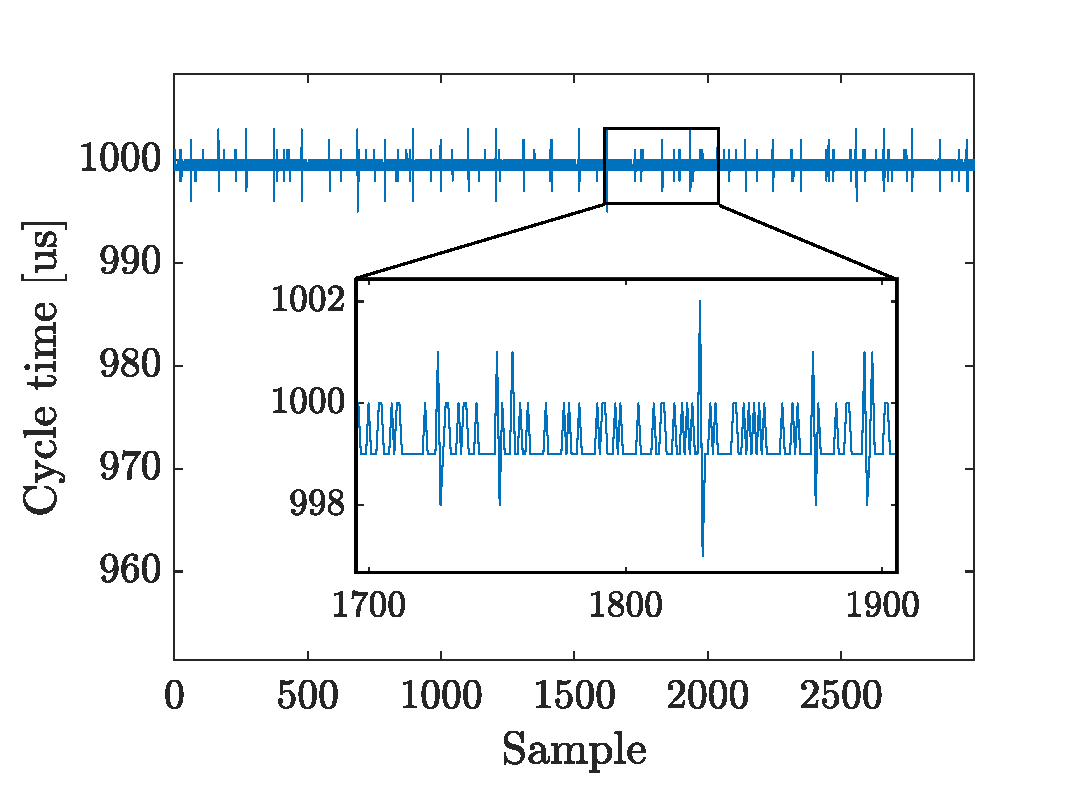
\includegraphics[width=.7\linewidth]{images/ch6/pub.eps}
  \caption{Steady-state cycle time of the real-time thread containing a \texttt{Publisher} \texttt{DDSDataSource} running in \texttt{Synchronized} mode.}
  \label{fig:ddsdatasource_benchmark_pub}
\end{figure}

\subsubsection{Subscriber side in Synchronized mode}
\label{sec:ddsdatasource_benchmark_subsync}
The steady-state cycle time of a real-time MARTe2 thread running the subscriber \texttt{DDSDataSource} in \texttt{Synchronized} mode is shown in \Cref{fig:ddsdatasource_benchmark_subsync}. Recall that in this mode the DataSource is synchronized with the transport layer and blocks the running thread, waiting until a new data packet has been received. Thus, the expected cycle time of the real-time thread in ideal conditions is that of the publisher thread, equal to \SI{1000}{\micro\second}. \Cref{fig:ddsdatasource_benchmark_subsync} shows that the actual cycle time averages to that value, but the jitter reaches considerable peaks of over \SI{100}{\micro\second}. This is due to the fact that each time the thread has to wait for a new data packet, it hands over control to the operating system: the thread is first removed from the run queue of its CPU, then it is put back in when a new data packet is received. This operation and all the context switches in between introduce non-deterministic latencies that, no matter how efficient and deterministic the kernel scheduler is, become noticeable when the timings have this order of magnitude. Thus, this behavior is expected and compliant with the \texttt{RFM2g} implementation but it is unavoidable and confirms that this execution mode suits data collection and offline diagnostics use cases.
\begin{figure}[t!]
  \centering
  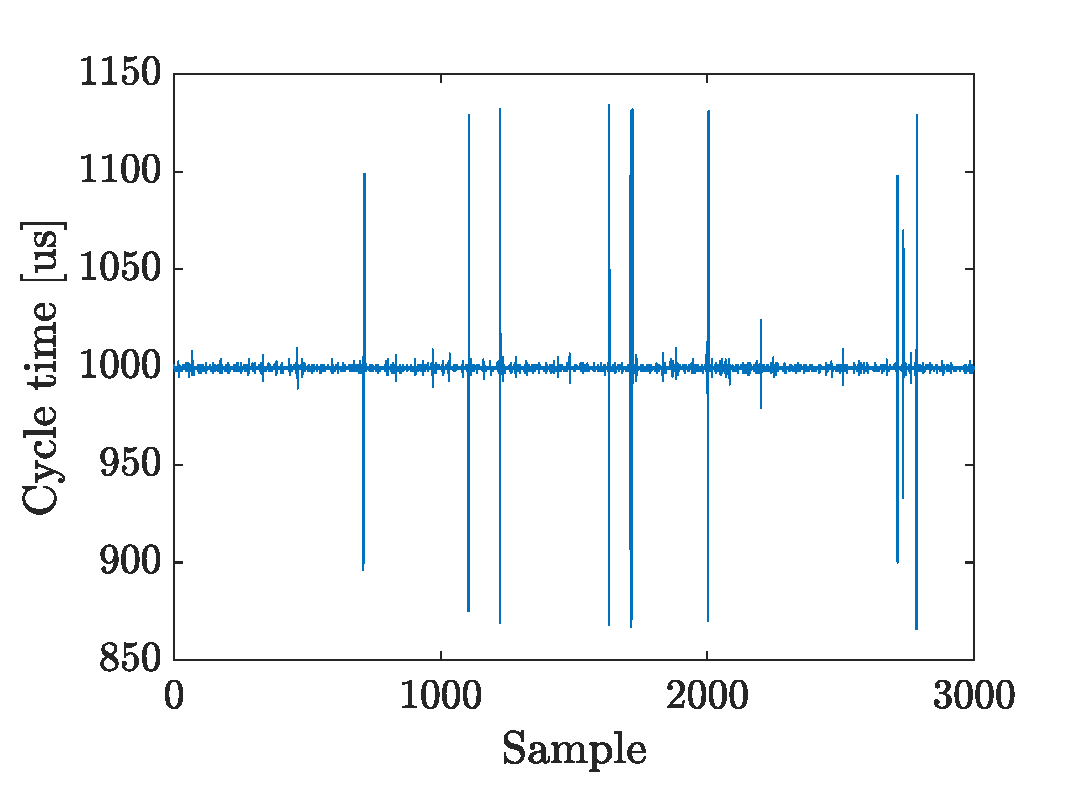
\includegraphics[width=.7\linewidth]{images/ch6/sub_sync.eps}
  \caption{Steady-state cycle time of the real-time thread containing a \texttt{Subscriber} \texttt{DDSDataSource} running in \texttt{Synchronized} mode.}
  \label{fig:ddsdatasource_benchmark_subsync}
\end{figure}

\subsubsection{Subscriber side in NotSynchronized mode}
\label{sec:ddsdatasource_benchmark_subasync}
\Cref{fig:ddsdatasource_benchmark_subasync} depicts the steady-state cycle time of a real-time MARTe2 thread running a subscriber \texttt{DDSDataSource} in \texttt{NotSynchronized} mode. Recall that, in this mode, the DataSource does not enforce a rate for the real-time thread loop, thus a \texttt{LinuxTimer} DataSource has been added to the tasks performed by the thread. The rate of the \texttt{LinuxTimer}, to test the capabilities of the implementation, has been pushed at \SI{5}{\kilo\hertz}: five times higher than that of the publisher, resulting in an expected cycle time of \SI{200}{\micro\second}. Note that, by configuring the real-time thread in this way and with this execution mode, the \texttt{DDSDataSource} copies and returns the same \SI{4}{\kilo\byte} sample five times for every publisher cycle. \Cref{fig:ddsdatasource_benchmark_subasync} shows that the actual cycle time is, in practice, compatible with the expected value: the maximum jitter observed at steady-state is equal to \SI{5}{\micro\second}, which is negligible compared to the overall cycle time. Moreover, the jitter is so small and periodic that it is fully compatible with the maximum time resolution achievable by the \texttt{LinuxTimer}, which is providing the clock to the entire real-time thread. This final test confirmed that the \texttt{DDSDataSource} implementation is also suitable for fast feedback control applications when configured in this way and confirmed it as a replacement for the \texttt{RFM2g} DataSource in the SCD architecture.
\begin{figure}[t!]
  \centering
  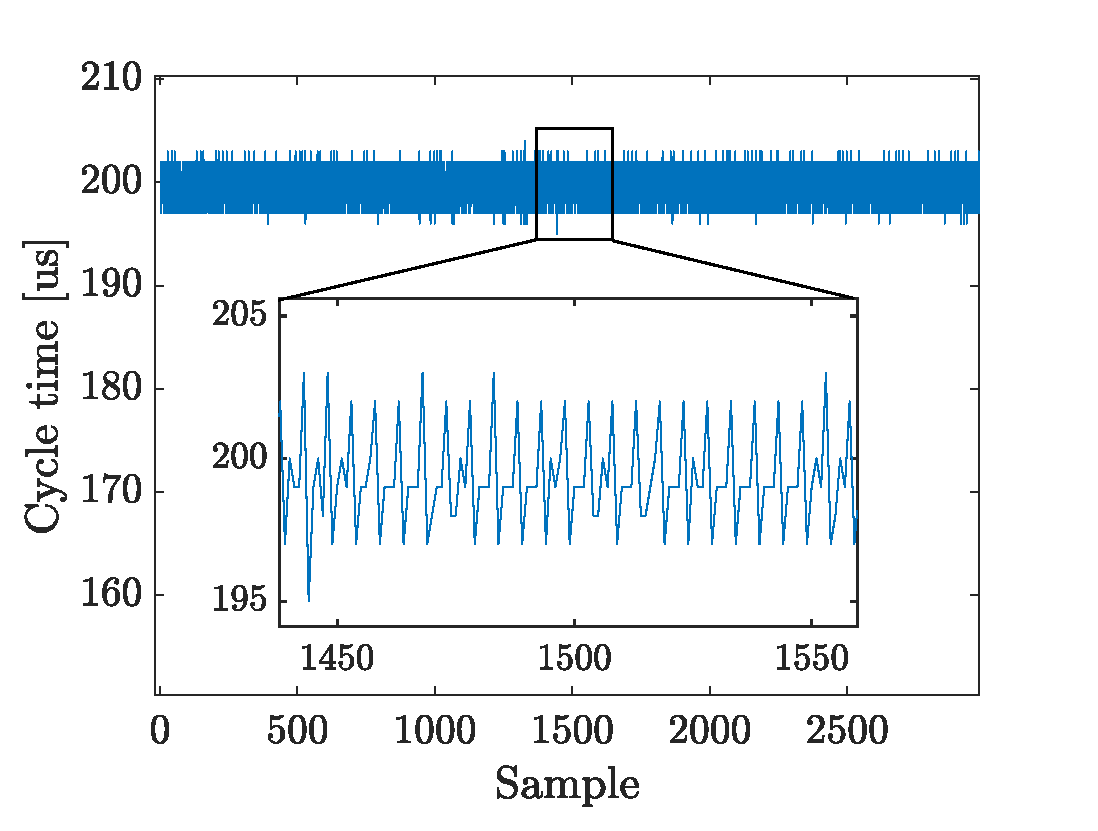
\includegraphics[width=.7\linewidth]{images/ch6/sub_async.eps}
  \caption{Steady-state cycle time of the real-time thread containing a \texttt{Subscriber} \texttt{DDSDataSource} running in \texttt{NotSynchronized} mode.}
  \label{fig:ddsdatasource_benchmark_subasync}
\end{figure}
